\documentclass[11pt,a4paper,oneside]{scrreprt}
\usepackage[utf8]{inputenc}
\usepackage[T1]{fontenc}
\usepackage[ngerman]{babel}
\usepackage{lmodern}
\usepackage{amsmath,amssymb}
\usepackage{graphicx}
\usepackage{booktabs}
\usepackage{array}
\usepackage{geometry}
\usepackage{hyperref}
\geometry{left=30mm,right=25mm,top=27mm,bottom=27mm}
\hypersetup{hidelinks,pdftitle={Statische strukturmechanische Ersatzmodelle}}
\setlength{\emergencystretch}{2em}
\graphicspath{{abbildungen/}}
% Persönliche Angaben vor Abgabe ergänzen. Kontakte aus der Aufgabenstellung
% werden nicht automatisch als zugewiesene Betreuung interpretiert.
\newcommand{\BerichtTitel}{Vergleich neuronaler und gaußprozessbasierter Ersatzmodelle für statische strukturmechanische Berechnungen}
\newcommand{\SeminarTitel}{Masterseminar I -- Angewandte Mathematik}
\newcommand{\AufgabenTitel}{Einsatz von Neuronalen Netzen als Ersatzmodell für strukturmechanische Berechnungen}
\newcommand{\AutorName}{[Name ergänzen]}
\newcommand{\Matrikelnummer}{[Matrikelnummer ergänzen]}
\newcommand{\Studiengang}{[Studiengang ergänzen]}
\newcommand{\Betreuung}{[Zugewiesene Betreuung ergänzen]}
\newcommand{\AbgabeDatum}{[Abgabedatum ergänzen]}

\begin{document}
\hypersetup{pageanchor=false}
\begin{titlepage}
\centering
{\large Technische Hochschule Ulm\par}
\vspace{1.5cm}
{\large \SeminarTitel\par}
\vspace{0.4cm}
{\normalsize \AufgabenTitel\par}
\vfill
{\LARGE\bfseries \BerichtTitel\par}
\vspace{0.8cm}
{\large Wissenschaftlicher Seminarbericht\par}
\vfill
\begin{tabular}{@{}ll@{}}
Verfasser/in: & \AutorName\\
Matrikelnummer: & \Matrikelnummer\\
Studiengang: & \Studiengang\\
Betreuung: & \Betreuung\\
Abgabe: & \AbgabeDatum
\end{tabular}
\vspace{2cm}
\end{titlepage}
\pagenumbering{Roman}
\hypersetup{pageanchor=true}
\chapter*{Kurzfassung}
\addcontentsline{toc}{chapter}{Kurzfassung}
Parametrisierte strukturmechanische Berechnungen können bei wiederholter Auswertung durch datengetriebene Ersatzmodelle beschleunigt werden. Diese Arbeit vergleicht ein direktes mehrschichtiges neuronales Netz (MLP), eine konkrete radiale Basisfunktionsvariante (RBF), ein POD--MLP und ein POD--GPR. Ausgangspunkt sind sechs Geometrie-, Material- und Lastparameter; vorhergesagt wird das vollständige statische Verschiebungsfeld an 525 Punkten mit drei Komponenten. Der Trainingspool umfasst 768 FEM-Fälle. Für die Modellwahl werden 128 neue Validierungsfälle und für die unabhängige Bewertung 256 Interpolations- sowie 128 Extrapolationsfälle verwendet.

Bei 768 Trainingsfällen beträgt der mittlere gewichtete relative Interpolationsfehler 4,64\,\% für das MLP, 7,41\,\% für die RBF-Variante, 4,78\,\% für POD--MLP und 0,55\,\% für POD--GPR. Für die definierte Extrapolation ergeben sich 16,24\,\%, 32,67\,\%, 13,74\,\% beziehungsweise 3,85\,\%. Die vollständige Fit-Zeit des ausgewerteten POD--GPR-Hauptmodells beträgt 353,57\,s und übersteigt die neuronalen Fit-Zeiten deutlich. Ein zusätzlicher Benchmark vergleicht vollständige Surrogatvorhersagen mit FEM-Lösung und Feldinterpolation auf zwölf vorab gewählten Fällen. Die daraus abgeleiteten Amortisationswerte sind bedingte Szenarien. Große relative Extrapolationsfehler treten insbesondere bei kleinen Referenznormen auf; zudem sind absolute Abweichungen und falsche Vorzeichen einzelner neuronaler Spitzenvorhersagen nachweisbar. Die Befunde gelten für das untersuchte lineare Balkenproblem und die begrenzten Such- und Testbereiche.

\tableofcontents
\cleardoublepage
\pagenumbering{arabic}
\chapter{Einleitung und Zielsetzung}
\section{Motivation und Fragestellung}
Die Finite-Elemente-Methode (FEM) ermöglicht die numerische Untersuchung strukturmechanischer Probleme, verursacht aber bei wiederholter Lösung unterschiedlicher Parameterkombinationen wiederkehrende Rechenkosten. Ein aus bereits berechneten Beispielen angepasstes Ersatzmodell kann die Parameter-Lösungs-Abbildung approximieren. Dem schnellen Online-Aufruf stehen die Kosten für Referenzdaten und Modellanpassung gegenüber. Die Aufgabenbeschreibung des Masterseminars schlägt dafür zunächst einen einseitig eingespannten Biegebalken und die statische Auslenkung als Ausgangspunkt vor\cite{aufgabe}.

Die Leitfrage dieser Arbeit lautet: Wie unterscheiden sich die untersuchten Ersatzmodelle hinsichtlich Genauigkeit vollständiger Verschiebungsfelder, Datenbedarf, Trainingsaufwand und Vorhersagezeit? Verglichen werden ein direktes MLP, die vorhandene RBF-Variante, POD--MLP und POD--GPR. Die Studie untersucht ausschließlich statische Verschiebungen; Eigenfrequenzen werden nicht ausgewertet. Die Bewertung erfolgt auf separaten Interpolations- und Extrapolationsfällen. Ein kleiner nachträglicher Benchmark ergänzt die ursprünglichen Messungen um einen begrenzten FEM-Vergleich.

\chapter{Grundlagen}
\section{Direktes Netz und radiale Basisfunktionen}
Ein mehrschichtiges Perzeptron bildet einen Eingabevektor durch aufeinanderfolgende affine Transformationen und nichtlineare Aktivierungen auf eine Ausgabe ab. Im direkten Ansatz besteht die Ausgabe aus allen 1575 Feldkomponenten. Die Netzbreite und -tiefe bestimmen die Architektur; Adam ist dagegen ein Optimierungsverfahren zur iterativen Anpassung der Gewichte\cite{kingma2015}. Eine gewichtete Feld-MSE misst im Training die Abweichung über das Feld, während die alternative Standardisierung einzelne Ausgabespalten skaliert.

Radiale Basisfunktionen ordnen Eingaben anhand ihrer Distanz zu Zentren Merkmale zu\cite{broomhead1988}. Die hier verwendete Implementierung berechnet zunächst Gaußmerkmale für feste Zentren und führt sie anschließend durch trainierbare Tanh-Schichten. Sie ist weder mit einem beliebigen RBF-Verfahren noch mit einer Optimierung der Zentren gleichzusetzen.

\section{Gewichtete Proper Orthogonal Decomposition}
Die Proper Orthogonal Decomposition (POD) bestimmt aus Beispielschnappschüssen einen niedrigdimensionalen linearen Raum\cite{sirovich1987}. Für einen zentrierten Feldvektor $u-\bar u$ und eine im Projekt verwendete positive Gewichtsmatrix $W$ gelten für die behaltenen Basisvektoren $\Phi_r$ die gewichtete Orthonormalität $\Phi_r^{\mathsf T}W\Phi_r=I$ und die Projektion
\begin{equation}
 a=\Phi_r^{\mathsf T}W(u-\bar u),\qquad
 \widehat u=\bar u+\Phi_r\widehat a.
 \label{eq:pod}
\end{equation}
Der Rang $r$ legt die Zahl der Koeffizienten fest. POD ist eine Dimensionsreduktion und kein neuronales Netz. Im POD--MLP lernt das Netz die Abbildung der Parameter auf $a$. Verwandte Forschungsarbeiten kombinieren reduzierte Lösungsräume und neuronale Modelle auch für parametrisierte partielle Differentialgleichungen; deren nichtlineare beziehungsweise zeitabhängige Aufgaben sind nicht identisch mit dem vorliegenden statischen Balken\cite{salvador2021,fresca2021}.

\section{Gaußprozessregression}
Ein Gaußprozess beschreibt eine Verteilung über Funktionen, deren endliche Auswertungen gemeinsam normalverteilt sind. Mittelwert- und Kovarianzfunktion bestimmen diese Verteilung\cite{rasmussen2006}. Beim POD--GPR wird für jeden nicht konstanten POD-Koeffizienten ein separates GPR-Modell trainiert. Die konkrete Implementierung verwendet exakte Anpassung mit \texttt{fitrgp}\cite{mathworks2025}. Die Eingaben und Koeffizienten werden anhand der Trainingsdaten standardisiert. Konstante Eingabespalten werden aus dem Prädiktor entfernt; konstante Ziele werden direkt rekonstruiert. Das feste numerische Sigma stabilisiert das Modell und wird hier nicht als Messrauschen interpretiert. Eine Kalibrierung der GPR-Unsicherheit ist nicht Gegenstand der Untersuchung.

\section{Fehlergrößen und POD-Zerlegung}
Für ein Referenzfeld $u$ und eine Vorhersage $\widehat u$ ist der gewichtete relative Feldfehler definiert als
\begin{equation}
 e_{\mathrm{rel}}=\frac{\lVert u-\widehat u\rVert_W}{\lVert u\rVert_W},
 \qquad \lVert v\rVert_W=\sqrt{v^{\mathsf T}Wv}.
 \label{eq:error}
\end{equation}
Die Größe ist ein Fehler des gesamten Feldes, keine punktweise Fehlerschranke. Bei kleiner Referenznorm kann sie trotz begrenzter absoluter Abweichung stark ansteigen. Ergänzend werden absolute Feldfehler sowie Fehler der Spitzenauslenkung und des maximalen Verschiebungsbetrags ausgewiesen.

Die orthogonale Projektion erlaubt eine fallweise quadratische Zerlegung des Feldfehlers in Projektions- und Regressionsanteil. Die in den Ergebnissen berichteten Mittelwerte relativer Wurzeln sind im Allgemeinen nicht additiv. P95 bezeichnet das nach der Nearest-Rank-Regel ermittelte 95. Perzentil der Fallfehler. Es beschreibt die Verteilung der beobachteten Fälle, keine garantierte Fehlerschranke.

\chapter{Referenzproblem und Datengrundlage}
Untersucht wird ein linear-elastischer Quaderbalken, der an einer Stirnfläche fest eingespannt und an der anderen durch eine gleichmäßig verteilte $z$-gerichtete Flächenlast beansprucht wird. Die Geometrie wird für jeden Fall neu vernetzt. Die FEM-Lösung wird auf ein gemeinsames normiertes Raster mit $21\times5\times5=525$ Punkten interpoliert. Ausgegeben werden die drei Verschiebungskomponenten in Metern. Für die Stützfläche wird im gemeinsamen Raster die bekannte homogene Verschiebungsrandbedingung gesetzt.

Die sechs Eingaben und ihre Trainingsgrenzen sind in Tabelle~\ref{tab:grenzen} angegeben. Der Trainingspool umfasst je 384 Fälle aus zwei Erzeugungsblöcken. Die Auswahlen sind blockausgeglichen und für die Größen 48, 96, 192, 384 und 768 verschachtelt. Drei Auswahlen dienen der Untersuchung kleinerer Trainingsmengen; bei 768 Fällen sind sie identisch. Für neuronale Vollpoolmodelle werden zusätzlich drei Initialisierungen betrachtet.
\begin{table}[htbp]\centering\caption{Parameter und Grenzen des Trainingsintervalls.}\label{tab:grenzen}
\begin{tabular}{llrr}\toprule Parameter & Einheit & Untergrenze & Obergrenze\\\midrule
Länge $L$ & m & 0,60 & 1,20\\ Breite $b$ & m & 0,06 & 0,10\\ Höhe $h$ & m & 0,08 & 0,14\\ Elastizitätsmodul $E$ & GPa & 70 & 210\\ Querkontraktionszahl $\nu$ & -- & 0,25 & 0,35\\ Kraft $F_z$ & N & $-1000$ & $-100$\\\bottomrule\end{tabular}\end{table}

Neben dem Trainingspool entstehen 128 neue Validierungs-, 256 Interpolations- und 128 Extrapolationsfälle. Validierungs- und Interpolationsparameter werden unabhängig innerhalb der Grenzen mittels Latin-Hypercube-Verfahren erzeugt. Ein Extrapolationsfall überschreitet genau eine Parametergrenze um 5--10\,\% der zugehörigen Intervallbreite. Die zwölf Parameter-/Seitengruppen enthalten je zehn oder elf Fälle. Parametervektoren werden gegen bekannte Designs und neue Kandidaten auf Überschneidungen in einer durch Intervallbreiten normierten Maximumsnorm mit Toleranz $10^{-10}$ geprüft.

Die FEM-Referenzen verwenden quadratische Elemente und den Netzdivisor 3. Fälle müssen physikalische und numerische Prüfungen einschließlich eines maximalen Auslenkungsverhältnisses von 0,02 erfüllen. Ein separater Pilot umfasst zwölf Extrapolationsfälle auf drei Netzstufen; er ist keine Garantie für Netzkonvergenz im gesamten Parameterraum. Euler--Bernoulli- und Timoshenko-Balkentheorie werden als Plausibilitätsreferenzen genutzt, nicht als exakte Lösungen aller Komponenten des dreidimensionalen Feldes.

\chapter{Methoden und Versuchsplanung}
\section{Konfigurationswahl und Datenrollen}
Die Modellauswahl erfolgt bei $N=384$ auf einer Trainingsauswahl und den 128 Validierungsfällen. Zielgröße ist der mittlere gewichtete relative Feldfehler. Bei Gleichstand folgen P95 und eine feste Konfigurationskennung; die zwei besten neuronalen Kandidaten werden mit drei Initialisierungen bestätigt. GPR wird nach einem deterministischen Protokoll abgestimmt. Für die Lernkurven bleibt danach je Familie dieselbe Konfiguration erhalten; eine separate Abstimmung je $N$ findet nicht statt. Abbildung~\ref{fig:ablauf} stellt die Trennung der Datenrollen dar.
\begin{figure}[htbp]\centering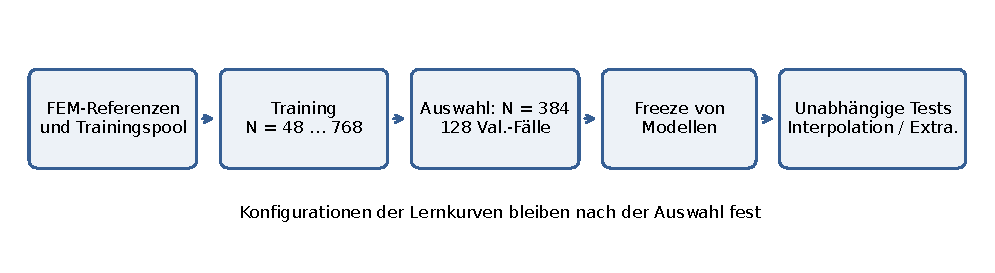
\includegraphics[width=\textwidth]{ablauf.pdf}\caption{Datenrollen und zeitliche Trennung der Modellwahl vom unabhängigen Test. Eigene Darstellung nach Studienprotokoll.}\label{fig:ablauf}\end{figure}

Die tatsächlich ausgewählten Einstellungen stehen in Tabelle~\ref{tab:config}. Die neuronalen Modelle verwenden Adam, höchstens 200 Epochen, eine Batchgröße von 32 und die Lernrate 0,001. GPR verwendet \texttt{ardmatern52}, einen linearen Mittelwert, ein konstantes numerisches Sigma von 0,001 und zwei Startlängenskalen. Die Quasi-Newton-Optimierung ist auf höchstens 500 Iterationen begrenzt. Der tatsächlich durchsuchte MLP-Raum umfasst Breiten 64 und 128, Tiefen 2 und 3, Lernraten 0,0005 und 0,001 sowie zwei Loss-Varianten; die ursprünglich vorgesehenen Breiten 32 und 80 fehlen.
\begin{table}[htbp]\centering\caption{Auf der Validierung ausgewählte Konfigurationen.}\label{tab:config}
\small\begin{tabular}{>{\raggedright\arraybackslash}p{25mm}>{\raggedright\arraybackslash}p{73mm}>{\raggedright\arraybackslash}p{30mm}r}\toprule Methode & Architektur beziehungsweise Kernel & Training / Loss & Rang\\\midrule
MLP & 3 Tanh-Schichten, Breite 128 & Adam, gew. Feld-MSE & --\\
RBF & 64 feste Gaußzentren, Breite 2; 2 Tanh-Schichten à 64 & Adam, gew. Feld-MSE & --\\
POD--MLP & 3 Tanh-Schichten, Breite 80 & Adam, gew. Feld-MSE & 2\\
POD--GPR & ARD-Matérn-5/2, linearer Mittelwert, Sigma 0,001 & exakte GPR & 15\\\bottomrule\end{tabular}\end{table}

\section{Kontrollierter POD- und Verteilungsvergleich}
Im kontrollierten POD-Vergleich werden die Ränge 2, 10 und 15 untersucht. POD--MLP und POD--GPR erhalten für denselben Rang, dieselbe Trainingsauswahl und Reihenfolge exakt denselben Mittelwert und dieselbe gewichtete Basis. Die Regressoreinstellungen der ausgewählten Familienkonfigurationen bleiben ansonsten fest. Die eigenständige Fit-Zeit wird als Summe aus der gemessenen Fit-Zeit mit vorbereiteter Basis und der separat gemessenen gemeinsamen POD-Zeit geschätzt.

Eine separate Untersuchung bei $N=192$ vergleicht eine raumfüllende mit einer auf niedrige Längen konzentrierten Auswahl. Beide sind blockausgeglichen und besitzen identische äußere Parametergrenzen. Die Bewertung erfolgt auf denselben unabhängigen Fällen.

\section{Freeze, Messung und Auswertung}
Vor Testlabelzugriff werden Konfigurationen, Daten- und Quellprüfsummen sowie die vorgesehenen Modellartefakte eingefroren. Die Tests werden anschließend getrennt nach Interpolation und Extrapolation ausgewertet. Die ursprüngliche Testauswertung brach nach dem ersten Modell wegen einer überschriebenen Manifestvariablen ab. Eine separat dokumentierte und gehashte technische Korrektur entstand nach dem ersten Testzugriff; Modelle, Auswahlregel und Metriken blieben unverändert. Für die beiden bereits berechneten Splits stimmen zwölf geprüfte numerische Fehler- und Referenzgrößen mit der Wiederholung überein. Die Korrektur ist somit dokumentiert, jedoch nicht nachträglich Teil des ursprünglichen Freeze.

Fit, Vorverarbeitung, POD beziehungsweise Zentrenaufbau, Regression, Suche sowie Laden und Speichern werden getrennt erfasst. Für vollständige Vorhersagen werden nach Warm-up wiederholte Einzelfall- und 128er-Batch-Aufrufe gemessen. Im Vollpool sind die drei neuronalen Wiederholungen unterschiedliche Netzinitialisierungen; zusätzliche deterministische GPR-Fits dienen ausschließlich der Zeitmessung.

Ein zusätzlicher, nachträglich angelegter Benchmark wählt vor der Messung zwölf Interpolationsfälle anhand fester Datenpositionen, unabhängig vom Vorhersagefehler. Auf derselben Maschine werden FEM-Lösung mit Feldinterpolation und vollständige Vorhersagen der eingefrorenen Modelle gemessen. Details und Kostenabgrenzung folgen in Kapitel~\ref{chap:ergebnisse}.

\chapter{Ergebnisse}\label{chap:ergebnisse}
\section{Genauigkeit bei 768 Trainingsfällen}
Tabelle~\ref{tab:fehler} und Abbildung~\ref{fig:genauigkeit} zeigen den vollständigen Feldfehler für die ausgewählten Familienkonfigurationen. Mittelwert und P95 werden je Lauf über Fälle bestimmt und für neuronale Modelle anschließend über drei Initialisierungen gemittelt. Das Maximum ist das größte tatsächlich beobachtete Fallmaximum über die jeweiligen Läufe. Für POD--GPR liegt ein deterministischer Vollpool-Hauptlauf vor; seine zwei zusätzlichen Fits sind Zeitwiederholungen, keine unabhängigen Datenziehungen.
\begin{table}[htbp]\centering\caption{Gewichteter relativer Feldfehler bei $N=768$. Angaben in Prozent.}\label{tab:fehler}
\small\begin{tabular}{lrrr rrr}\toprule
& \multicolumn{3}{c}{Interpolation} & \multicolumn{3}{c}{Extrapolation}\\
\cmidrule(lr){2-4}\cmidrule(lr){5-7} Methode & Mittel & P95 & Max. & Mittel & P95 & Max.\\\midrule
MLP & 4,64 & 14,78 & 58,59 & 16,24 & 50,74 & 638,23\\
RBF & 7,41 & 22,57 & 97,21 & 32,67 & 102,03 & 1253,55\\
POD--MLP & 4,78 & 15,73 & 43,78 & 13,74 & 47,82 & 286,56\\
POD--GPR & 0,55 & 2,20 & 6,65 & 3,85 & 15,85 & 88,55\\\bottomrule\end{tabular}\end{table}
\begin{figure}[htbp]\centering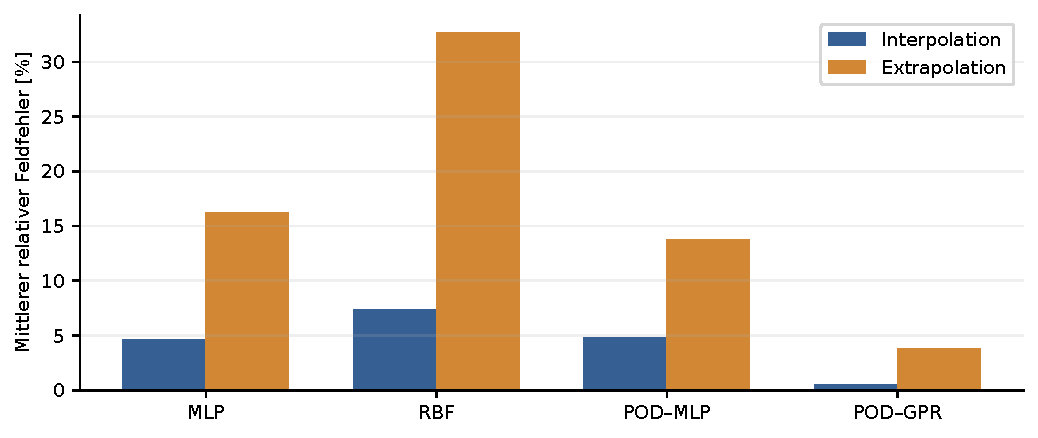
\includegraphics[width=.88\textwidth]{genauigkeit.pdf}\caption{Mittlerer relativer Feldfehler bei $N=768$. Neuronale Werte sind Mittel über drei Initialisierungen; POD--GPR umfasst einen Hauptlauf. Eigene Darstellung der Studienergebnisse.}\label{fig:genauigkeit}\end{figure}
POD--GPR erzielt auf beiden untersuchten Testverteilungen den kleinsten mittleren Fehler. Der Unterschied zwischen Interpolations- und Extrapolationsfällen ist bei allen Methoden deutlich. Auch für POD--GPR liegt das beobachtete Extrapolationsmaximum bei 88,55\,\%; der Mittelwert allein beschreibt die Randfälle folglich nicht ausreichend.

Für die Spitzenauslenkung am normierten Punkt $(1;0{,}5;0{,}5)$ beträgt der mittlere absolute Fehler bei POD--GPR 0,0007\,mm für Interpolation und 0,0023\,mm für Extrapolation. Beim direkten MLP sind es 0,0057 beziehungsweise 0,0106\,mm. Diese Punktgrößen ergänzen, aber ersetzen den vollständigen Feldfehler nicht.

\section{Datenbedarf und Trainingszeit}
Abbildung~\ref{fig:lernkurven} zeigt die Interpolationslernkurven und die mediane vollständige Fit-Zeit pro untersuchter Trainingsgröße. Die Konfigurationen wurden bei $N=384$ gewählt und bleiben über die Größen fest. Bei $N=192$ beträgt der mittlere Interpolationsfehler 5,58\,\% für MLP, 11,22\,\% für RBF, 9,71\,\% für POD--MLP und 2,69\,\% für POD--GPR. Bei $N=48$ treten teilweise sehr große Fehler und erhebliche Unterschiede zwischen Trainingsauswahlen auf. Bei $N=768$ unterscheiden sich die neuronalen Vollpoolläufe durch ihre Initialisierung, nicht durch verschiedene Vollpool-Daten.
\begin{figure}[htbp]\centering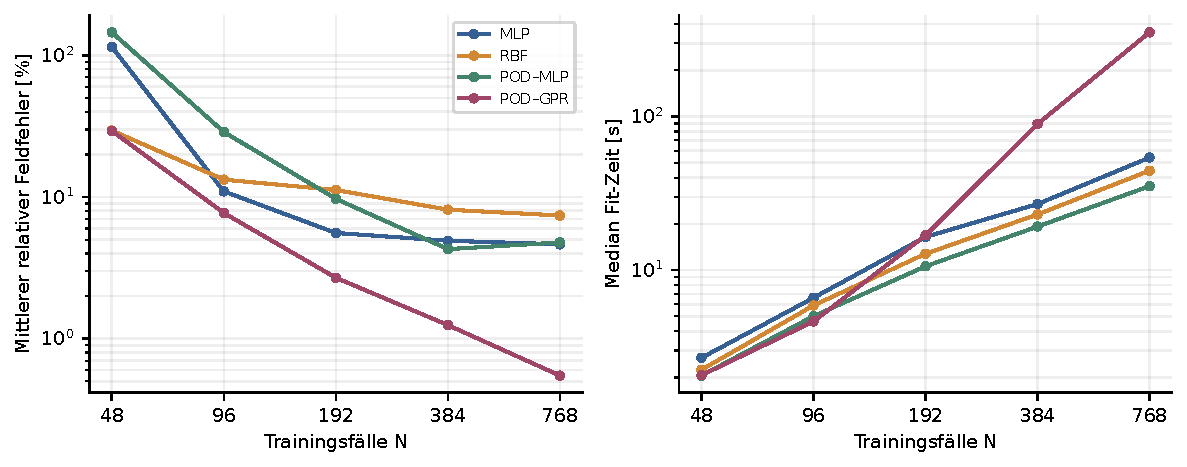
\includegraphics[width=\textwidth]{lernkurven.pdf}\caption{Mittlerer Interpolationsfeldfehler und mediane öffentliche Fit-Zeit gegen die Trainingsgröße. Logarithmische Achsen. Die Konfigurationen wurden bei $N=384$ festgelegt; die Art der Wiederholung ändert sich beim Vollpool. Eigene Darstellung.}\label{fig:lernkurven}\end{figure}

Die Fit-Zeit des ausgewerteten POD--GPR-Hauptmodells beträgt 353,5687942\,s. Zwei weitere Fits derselben Konfiguration dauern 337,1902846\,s und 336,1487963\,s. Der Median dieser drei vergleichbaren Zeitmessungen beträgt 337,1902846\,s; Trainingsfälle, Konfiguration und Fingerprints stimmen überein. Der Median ist somit nicht die Fit-Zeit des einzelnen ausgewerteten Hauptmodells. Die Zeiten umfassen den öffentlichen Fit, aber weder Speichern noch Validierungsvorhersage. Die Fit-Zeiten der neuronalen Seed-42-Hauptmodelle betragen 52,67\,s, 43,71\,s und 32,26\,s für MLP, RBF und POD--MLP.

\section{Einfluss der Trainingsverteilung}
Abbildung~\ref{fig:verteilung} zeigt bei $N=192$ den separaten Vergleich einer raumfüllenden und einer auf kleine Längen konzentrierten Auswahl. Die raumfüllende Auswahl erreicht für alle vier untersuchten Familien den geringeren mittleren Interpolationsfehler. Beispielsweise ergeben sich für POD--GPR 2,90\,\% gegenüber 5,08\,\%. Gleiche äußere Parametergrenzen bedeuten somit nicht notwendig eine vergleichbare Abdeckung im Inneren. Es handelt sich um die konkret untersuchten Designs, nicht um eine allgemeine Aussage über jede mögliche Verteilung.
\begin{figure}[htbp]\centering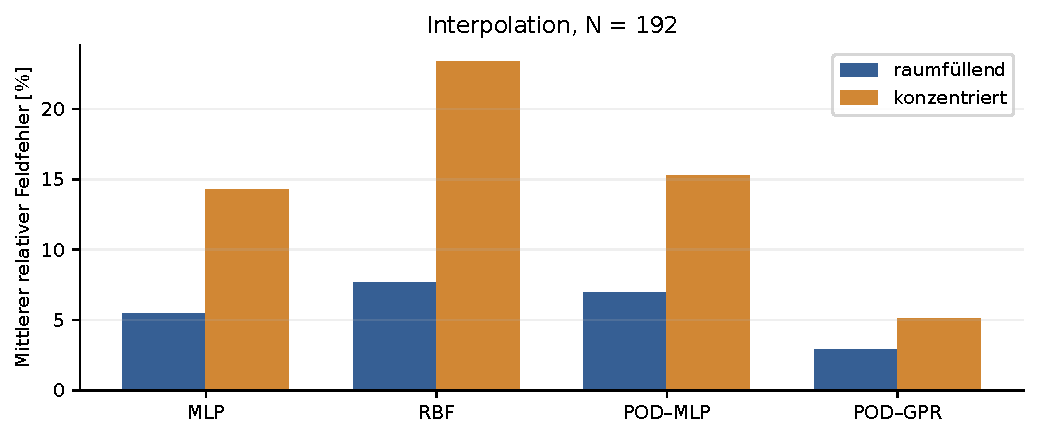
\includegraphics[width=.86\textwidth]{verteilung.pdf}\caption{Einfluss der Trainingsverteilung bei $N=192$ auf dieselben Interpolationsfälle. Eigene Darstellung der separaten Verteilungsstudie.}\label{fig:verteilung}\end{figure}

\section{POD-Rang, Fehleranteile und Aufbauaufwand}
Abbildung~\ref{fig:pod} zeigt den Projektions- und Koeffizientenregressionsanteil sowie die geschätzte eigenständige Fit-Zeit für die drei Ränge im kontrollierten Vollpoolvergleich. Beide Methoden verwenden dieselbe Basis pro Rang. Es handelt sich je Methode und Rang um einen Lauf, nicht um ein Mittel über neuronale Initialisierungen. Für POD--GPR beträgt der vollständige Interpolationsfehler bei Rang 2 beziehungsweise 15 0,560\,\% beziehungsweise 0,549\,\%; die entsprechenden eigenständigen Fit-Schätzungen sind 70,53\,s und 348,22\,s. Für die Extrapolation ergeben sich 3,861\,\% und 3,854\,\%. Die Unterschiede sind deskriptiv und nach Testeinsicht ermittelt.
\begin{figure}[htbp]\centering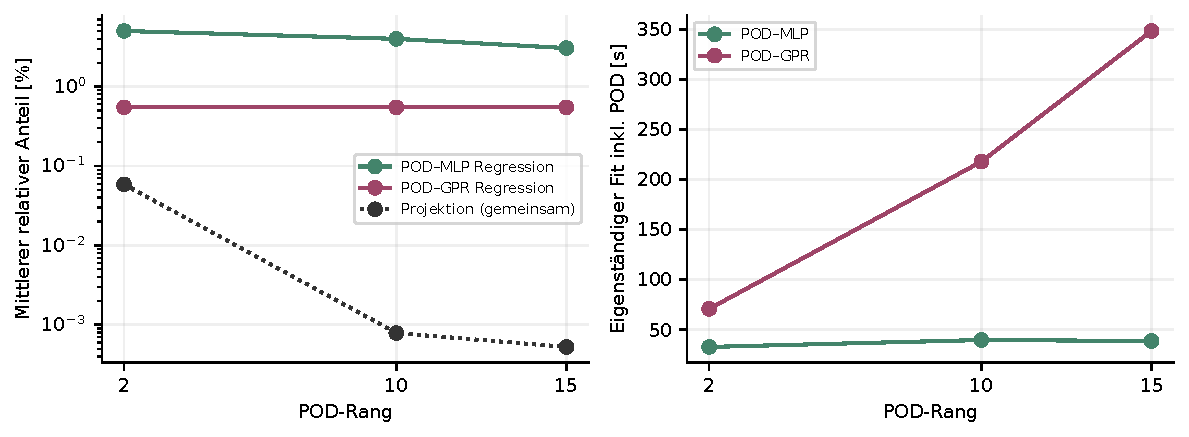
\includegraphics[width=\textwidth]{pod_rang.pdf}\caption{Kontrollierter POD-Vollpoolvergleich: mittlere relative Projektions- und Regressionsanteile für Interpolation sowie eigenständiger Fit einschließlich separat gemessener POD-Kosten. Ein Lauf je Rang und Methode; logarithmische Fehlerachse. Eigene Darstellung.}\label{fig:pod}\end{figure}

\section{Extrapolationsausreißer}
Der größte beobachtete relative Vollpoolfehler aller vier Familien betrifft Fall 830644. Der extrapolierte Parameter ist $F_z=-29{,}9502$\,N, oberhalb der Trainingsgrenze $-100$\,N und um 7,7833\,\% der Trainingsintervallbreite entfernt. Die Referenznorm beträgt $5{,}076\cdot10^{-7}$\,m. Der größte relative Fehler je Familie beträgt 638,23\,\% für MLP, 1253,55\,\% für RBF, 286,56\,\% für POD--MLP und 88,55\,\% für POD--GPR. Die Maxima von MLP und RBF stammen von anderen Initialisierungen als Seed 42.

Abbildung~\ref{fig:ausreisser} vergleicht für denselben Fall die vorab festgelegten Seed-42-Hauptmodelle. Die FEM-Spitze liegt bei $-0{,}001033$\,mm. Die direkte MLP-, RBF- und POD--MLP-Vorhersage besitzen dort ein falsches positives Vorzeichen; POD--GPR sagt $-0{,}001955$\,mm vorher. Die jeweiligen absoluten Feldfehler sind ungleich null. Unter den 13 größten relativen Fehlern je Seed-42-Modell liegen sieben, neun, sechs beziehungsweise acht Fälle in der zehn Fälle umfassenden Gruppe $F_z$ oberhalb der Grenze. Der Median der Referenznorm über alle 128 Extrapolationsfälle beträgt $5{,}04\cdot10^{-5}$\,m und ist damit deutlich größer als die typischen Normen der größten relativen Fehler. Niedrige Referenznormen verstärken die relative Kennzahl; sie erklären jedoch nicht alle absoluten Feldabweichungen.
\begin{figure}[htbp]\centering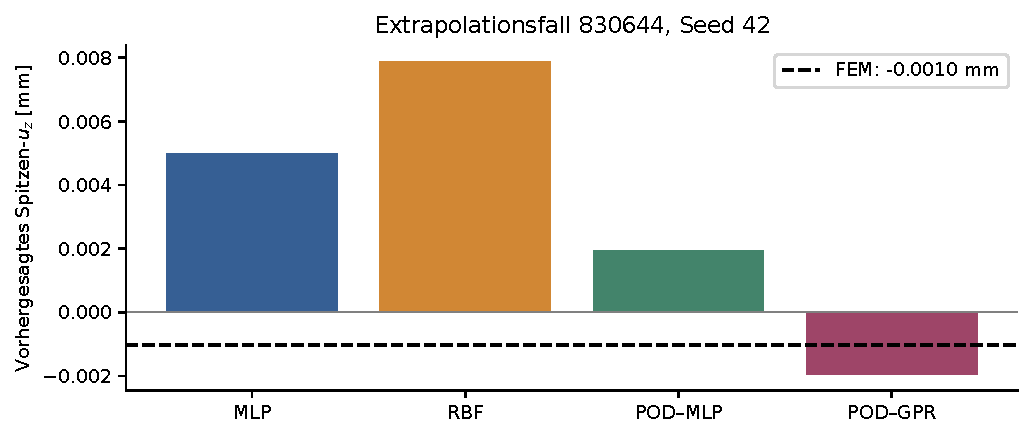
\includegraphics[width=.85\textwidth]{ausreisser.pdf}\caption{Vorhergesagtes vorzeichenbehaftetes Spitzen-$u_z$ des Extrapolationsfalls 830644 für die Seed-42-Hauptmodelle. Die gestrichelte Linie zeigt die FEM-Referenz. Eigene Darstellung.}\label{fig:ausreisser}\end{figure}

\section{Zusätzlicher FEM- und Vorhersagebenchmark}
Der nachträgliche Benchmark verwendet zwölf vorab unabhängig vom Fehler gewählte Interpolationsfälle auf einem AMD Ryzen 5 4500U unter MATLAB R2025b. Nach einem FEM-Warm-up werden die Fälle je zweimal seriell gelöst, im zweiten Durchlauf in umgekehrter Reihenfolge. Der FEM-Aufruf umfasst Geometrie, Netz, Lösung, vollständige Feldinterpolation sowie Spitzenabfrage und Prüfungen. Für die eingefrorenen Seed-42-Modelle werden nach Warm-up 30 vollständige Einzelfallaufrufe pro Fall und 30 gemeinsame 12er-Batches gemessen. Das Laden wird getrennt erfasst; Dateizugriffe sind aus den eigentlichen Vorhersagezeiten ausgeschlossen.

Der Median der fallweisen FEM-Mediane beträgt 2,189\,s; der Interquartilsabstand zwischen Fällen beträgt 1,734\,s. Die Summe der zwölf fallweisen FEM-Mediane ist 29,418\,s und keine Messung eines optimierten FEM-Batchsolvers. Abbildung~\ref{fig:zeiten} zeigt die Surrogatzeiten. Beim Einzelfall liegen sie zwischen 7,573 und 9,252\,ms; beim gemeinsamen 12er-Aufruf zwischen 9,835 und 18,469\,ms. FEM enthält zusätzliche Spitzenabfragen und Prüfungen; die Messumfänge sind deshalb nicht völlig identisch.
\begin{figure}[htbp]\centering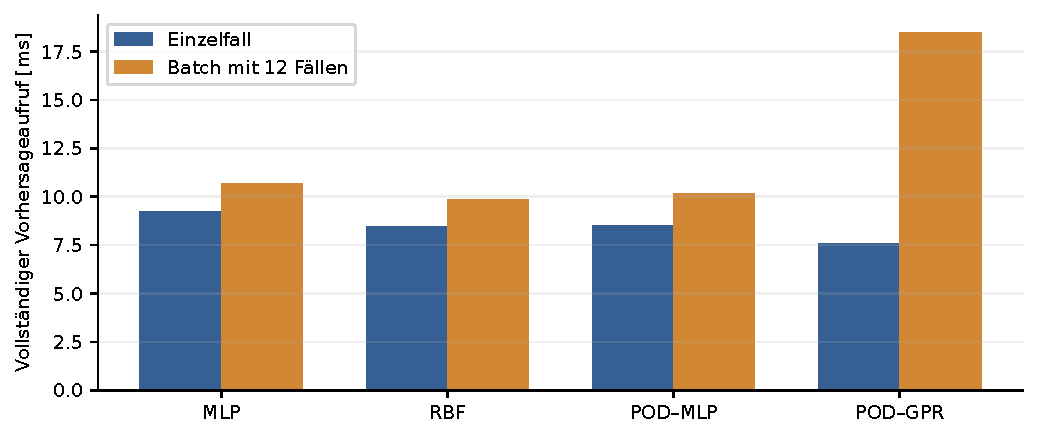
\includegraphics[width=.85\textwidth]{vorhersagezeit.pdf}\caption{Median vollständiger Surrogataufrufe im nachträglichen Benchmark: ein Fall und gemeinsamer 12er-Batch. Ladezeiten sind ausgeschlossen. Eigene Darstellung.}\label{fig:zeiten}\end{figure}

\section{Bedingte Amortisationsszenarien}
Für einen positiven Zeitgewinn pro Einzelfall wird die rechnerische Schwelle bestimmt durch
\begin{equation}
 Q_{\mathrm{BE}}=\left\lceil\frac{C_{\mathrm{offline}}}{t_{\mathrm{FEM}}-t_{\mathrm{Surrogat}}}\right\rceil.
\end{equation}
Mit vorhandenen Trainings- und Validierungsdaten umfasst $C_{\mathrm{offline}}$ hier den Fit des Seed-42-Hauptmodells, wahlweise zuzüglich äußerer Familiensuche. Für POD--GPR ergeben sich 163 Einzelfälle mit Fit beziehungsweise 714 mit Fit und Suche. Im seriellen FEM-/12er-Batch-Szenario sind es 156 beziehungsweise 636 Fälle. Fit und Suche stammen aus der Hauptstudie, Vorhersage- und FEM-Zeiten aus dem späteren Benchmark auf derselben Maschine. Die Werte sind bedingte Szenarien auf Medianbasis, ohne Unsicherheitsintervall und ohne Lade-, Speicher- oder Qualitätssicherungskosten.

Für eine hypothetische Neuerzeugung wird lediglich eine gemischte historische Rechenannahme aus 1632,92\,s Trainings-Solverzeit und 566,11\,s aktiver Validierungserzeugung angesetzt. Die Trainings-Gesamtzeit fehlt; diese Summe ist keine neu kontrolliert gemessene vollständige Datenerzeugung. Testdatenerzeugung, Pilot und weitere Studienkosten bleiben in den Szenarien unberücksichtigt. Die vollständigen methodenspezifischen Zahlen und Kostenabgrenzungen stehen im Anhang.

\chapter{Diskussion}
Die Ergebnisse zeigen für die konkret gewählten Konfigurationen einen deutlichen Genauigkeitsvorteil von POD--GPR. Dies ist keine allgemeine Überlegenheit von Gaußprozessen: Die Aussage betrifft einen begrenzten Parameterraum, ein linear-elastisches Referenzproblem und die durchsuchten Modell- und Hyperparameterräume. Das direkte MLP wurde nur für die Breiten 64 und 128 untersucht; die ursprünglich vorgesehenen Breiten 32 und 80 fehlen. Das Ergebnis der RBF-Familie betrifft feste Gaußzentren und nachgeschaltete Tanh-Schichten.

Im kontrollierten Vollpoolvergleich ist der Projektionsfehler bereits bei Rang 2 klein. Dass der vollständige POD--GPR-Fehler bei höheren Rängen nur geringfügig sinkt, legt einen günstigen Kompromiss bei kleinem Rang nahe. Diese Interpretation entstand nach Einsicht in die Testdaten. Sie ist eine Folgehypothese und ändert nicht den auf der Validierung gewählten Rang 15. Bei POD--MLP verändern sich die Fehler je Rang anders; aus einzelnen kontrollierten Läufen sollte nicht auf die gesamte Verteilung möglicher neuronaler Initialisierungen geschlossen werden.

Die Extrapolationsfälle überschreiten jeweils nur eine Grenze. Die großen relativen Fehler bei kleiner Referenznorm sind nicht gleichbedeutend mit gleich großen absoluten Fehlern. Umgekehrt zeigen die absoluten Fehler und falschen Vorzeichen im auffälligen Lastfall, dass die relativen Ausreißer nicht allein ein Effekt der Normierung sind. Die nachträgliche Gruppenauswertung enthält nur zehn oder elf Fälle pro Gruppe und erlaubt keine gesicherte Ursachenzuordnung.

Die FEM-Felder sind Referenzen des verwendeten numerischen Netzes. Die Netzuntersuchung im Pilot ist begrenzt; eine flächendeckende Konvergenzprüfung liegt nicht vor. Analytische Balkentheorien dienen als Plausibilisierung und beschreiben nicht alle Komponenten des dreidimensionalen Feldes exakt. Die unabhängigen Testfälle sind in ihrer Rolle von der Validierung getrennt, wurden jedoch über dieselben Modelle wiederholt vorhergesagt; Seeds erzeugen keine zusätzlichen unabhängigen Balkenfälle.

Die technische Auswertekorrektur nach dem ersten Testzugriff ist eine Einschränkung der ursprünglichen Vorabprovenienz. Ihr Änderungsumfang, die unveränderten Modelle und Kennzahlen sowie der Vergleich der ersten beiden Split-Ergebnisse sind separat dokumentiert. Für POD--GPR wurde keine Unsicherheitskalibrierung vorgenommen; der Spitzen-RAM wurde nicht gemessen. Die Laufzeit- und Break-even-Werte hängen von Messumfang, Rechner, Datenkosten und Aufgabenverteilung ab. Der kleine spätere Benchmark erlaubt eine bedingte Szenariorechnung, nicht die Behauptung einer universellen Schwelle.

\chapter{Fazit und Ausblick}
Für den vorliegenden statischen Vergleich ist POD--GPR bei $N=768$ der genauigkeitsorientierte Ausgangspunkt: Der mittlere Interpolationsfehler beträgt 0,55\,\% und der mittlere Extrapolationsfehler 3,85\,\%. Dem steht eine vollständige Fit-Zeit des ausgewerteten Hauptmodells von 353,57\,s gegenüber. POD--MLP ist schneller trainiert, erreicht aber einen größeren Feldfehler. Direkte MLP- und RBF-Modelle sind weitere Bezugspunkte, deren Ergebnisse von ihrem begrenzten Suchraum abhängen. Der Datenbedarf wird nicht allein durch die Fallzahl bestimmt: Die separate Verteilungsstudie zeigt für alle vier Familien einen Vorteil des konkret betrachteten raumfüllenden Designs.

Für weiterführende Arbeiten bietet sich eine vorab definierte Untersuchung kleiner POD-Ränge mit neuen unabhängigen Bewertungsfällen an. Ebenso können Netzkonvergenz, kritische Lastfälle und eine mögliche Kalibrierung der GPR-Unsicherheit vertieft werden. Eine Erweiterung auf Eigenfrequenzen wäre ein eigenständiger nächster Schritt und ist nicht durch die statischen Ergebnisse dieser Arbeit belegt.

\bibliographystyle{unsrt}
\bibliography{literatur}
\appendix
\chapter{Ergänzende Tabellen und Reproduzierbarkeit}
\section{Aufwand und bedingte Einzelfallszenarien}
Tabelle~\ref{tab:break} enthält die Familiensuche und die berechneten Einzelfallschwellen für bereits verfügbare Trainings- und Validierungsdaten. Die Randbedingungen und die Grenzen der Szenarien sind in Kapitel~\ref{chap:ergebnisse} erläutert.
\begin{table}[htbp]\centering\caption{Bedingte Szenarien bei bereits verfügbaren Daten: Seed-42-Fit, äußere Familiensuche und rechnerische Einzelfallschwellen.}\label{tab:break}
\small\begin{tabular}{lrrrr}\toprule Methode & Fit [s] & Suche [s] & Fälle: Fit & Fälle: Fit + Suche\\\midrule
MLP & 52,67 & 721,25 & 25 & 356\\
RBF & 43,71 & 708,47 & 21 & 346\\
POD--MLP & 32,26 & 299,29 & 15 & 153\\
POD--GPR & 353,57 & 1203,16 & 163 & 714\\\bottomrule\end{tabular}\end{table}

\section{Daten- und Quellnachweise}
Die Abbildungen dieses Berichts wurden aus den kopierten Tabellen im Unterordner \texttt{daten} mit \texttt{skripte/diagramme.py} erzeugt. Die ursprünglichen Falltabellen, Modelle, Suchhistorie, das Studienprotokoll und die Checkpoints verbleiben in den zugehörigen Projektordnern der Hauptstudie. Der ergänzende Seminarbericht und die Benchmark-Rohdaten liegen im separaten Ergänzungsordner. Die Kopien in diesem Bericht dienen dem portablen Nachvollzug der gezeigten Diagramme; sie ersetzen nicht die vollständige Studienprovenienz.

Die Hauptstudie enthält 288 erfolgreiche Lauf-/Split-Auswertungen und 55.296 Fallzeilen. Dieselben Testfälle werden über mehrere Modelle wiederholt ausgewertet; die Zeilen sind daher keine 55.296 unabhängigen Balkenfälle. Die Studienauswertung zählt keine fehlgeschlagenen Lauf-/Split-Auswertungen und keine undefinierten relativen Fallfehler.

\end{document}
